\section{Tentris}
\label{sec:preliminaries:tentris}

There is no standard design guideline for triple stores. Hence different implementations of triple stores co-exist. Each subgroup of these implementations utilizes a category of underlying data structures and corresponding algorithms to govern the structures' behaviors. 
In production, triple stores are used to store up to billions of RDF triples. 
To that extent, quality factors like efficiency and scalability are considered first-class citizens during triple stores' construction. 
The selection of internal data structures and the behavior definitions greatly influence the overall system efficiency. \\

Fuseki, Blazegraph, Virtuoso, and RDF-3X are popular implementations of Triple stores \cite{fouc,SYS13,Erl,rdf3x}. 
One of the key design characteristics those triple stores have in common is that they all utilize B+ trees to store triples' representations. 
Other categories of triple stores use 3D Boolean tensors to store and process RDF data. Examples of such system include TensorRDF \cite{tensorrdf} and BitMat \cite{bitmat}. In such systems, each tensor dimension is mapped to a triple data aspect, i.e., subject, predicate, or object. Examples of tensor-based triple stores include systems like TensorRDF and BitMat. In the following, a novel tensor-based RDF triple store is presented. \\

Tentris is a triple store variant designed by the data science research group at Paderborn university\cite{tentris2020}. 
Tentris is an in-memory storage solution that represents RDF knowledge graphs as sparse order-3 tensors using a novel data structure, called Hypertire. 
It then uses tensor algebra to carry out SPARQL queries by mapping SPARQL operations to tensor operations, namely slicing and Einstein summation\cite{einstein}. 
At the time of this writing, Tentris' SPARQL engine realizes \textit{SPARQL-BGB}  (a subset of the SPARQL-algebra). 
Consequently, the engine can execute SPARQL queries containing the following keywords: \verb|SELECT|, \verb|WHERE|, and \verb|DISTINCT|\cite{Hitzler}. \\

Since this work represents a further contribution to the project Tentris, this section is dedicated to delivering a preface for the Tentris system design aspects. In sub-section \ref{sec:tensor_algebra}, I specify what tensors are. A way of representing RDF graphs in tensors is showed in sub-section \ref{sec:rdf_tensor}. Hypertrie data structure is visited in sub-section \ref{sec:hypertrie}.

\subsection{Tensor Algebra}
\label{sec:tensor_algebra}
In mathematics, the term \textit{tensor} holds a representation-independent meaning. According to \cite{rent}, tensors are “objects with many indices that transform in a specific way under a change of
Basis”. This mathematical construct has many applications in physics, artificial intelligence, and other fields. However, to apply tensors in a practical context, a more concrete definition should be selected. Among other choices, a multi-dimensional array is widely adopted as a representation of a tensor. Throughout this work, a finite $n$-dimensional array for tensor representation is considered.
In the context of the Tentris project \cite{tentris2020}, the term tensor has the following formal definition:

\begin{definition}[Tensor]
A mapping\\
\centerline{$T: \textbf{K} \to V$}\\
from a multi-index $\textbf{K}$ to a codomain $V$ is called tensor. $\textbf{K}$ is called \textit{key basis} of dimension $n \in \mathbb{N}$ with \\
\centerline{ $\textbf{K} = K_0 \times K_1 \times ... \times K_{n-1}, K_i \subset \mathbb{N}$ } \\
The tuple $\textbf{k} \in \textbf{K}$ is called \textit{key}, $K_i$ is called a \textit{key part basis} and $k \in K_i$ is called \textit{key part}.\\
The dimension of the key basis is also called dimension of the tensor and is denoted by ndim($T$)=$n$. Further, nnz($T$) = $|\{\textbf{k} \in \textbf{K} | T(\textbf{k})  \neq 0\}|$ denotes the \textit{ number of non-zero entries} in tensor $T$.
\end{definition} 

To resolve a value of a tensor, we use the array subscript notation $T[k_0, .. , k_{n-1}]$. Moreover, the symbol $V^{\textbf{K}}$ denotes the set of all mappings $T: \textbf{K} \to V$. My work exclusively consider tensors $T$ with $\mathbb{B}$ or $\mathbb{N}$ as codomain and only use multi-indexes with equal key part basis $K_1 = ... = K_n \subset \mathbb{N}$. An $n$-dimensional tensor is also called \textit{order-$n$} tensor.
\begin{example}
\label{tensors_examples}
 In the following, some examples to illustrate the Definition 2.3:

\begin{enumerate}
	\item A tensor $S \in \mathbb{Z}^{\emptyset}$ is called a \textit{scalar}.\\
	\centerline{$S = 1$}
	So $S[\emptyset] = S[]$ is 1.
	\item A tensor $X \in \mathbb{Z}^{\mathbb{N}_3}$ is called a \textit{vector}.\\
	\centerline{$X =\left[ \begin{array}{c}
		4 \\ 7 \\ 15\\
		\end{array}\right]$}\\
	where $X[2]$ is 15. 
	\item Now, we take a three dimensional tensor $Y \in \mathbb{Z}^{\mathbb{N}_2 \times \mathbb{N}_2 \times \mathbb{N}_2}$. It can be visualized by a vector for the first key part which, in turn, has matrices each with dimensions corresponding to second and third key parts. As an example:\\
	\centerline{$Y = \left[ 
		\begin{array}{c}
		\left[\begin{array}{cc}  1 & 2 \\ 3 & 5 \\\end{array} \right]\\ 
		\left[\begin{array}{cc} 7 & 11 \\ 13 & 15 \\\end{array} \right]\\ 
		\end{array}
		\right]$}\\
	Such that, $Y[1, 0, 1]$ is 11.
\end{enumerate}
\end{example}

\subsubsection{Tensor Operations}
\label{sec:tensor_operations}
This section highlights the core operations on tensors. In particular, I describe what tensor slicing and Einstein summations are. In the following, formal definitions of the operations are skipped. Instead, the section presents them informally with examples.


\paragraph{Slices} Slicing is a useful operation to retrieve a well-defined portion of a tensor $T \in V^{K}$ in the form of a lower order tensor. Slicing is done by using a \textit{slice key} $\textbf{s} \in S = (K_0 \cup \{:\}) \times .... \times ( K_{n-1}\cup \{:\})$, and denoted like as we are retrieving a value but with one or more dimensions not bound, e.g. $T[:, x, :]$ (or $T[<:, x, :>]$). 
When applying slice key $\textbf{s}$ to a tensor $T$, the unbounded dimensions in the slice key (the ones that are marked with $:$) are kept. 
A slice key part $s_i \neq :$ removes
all entries with other key parts at position $i$ and removes $K_i$ from the resultant tensor domain. e.g., $T[:, 2, :]$ or $T[<:, 2, :>]$.

\begin{example}
	\label{ex:tensor_slicing}
	Back to the third item in Example \ref{tensors_examples}, slicing tensor $Y$ by slice keys $s_1 = <:, 1, :>$ results in an order-2 tensor $Z_1 = Y[:, 1, :]$, and with a slice key $s_2 = <0, 1, :>$ results in an order-1 tensor $Z_2 = Y[0, 1, :]$:\\
	
	 \centerline{$Z_1 = \left[ \begin{array}{cc} 3 & 5\\ 13 & 15 \\ \end{array}\right]$}  
	 
	 
	 \centerline{$Z_2 = \left[ \begin{array}{c} 3 \\ 5 \\ \end{array}\right]$} 
\end{example}

Worth to mention that, slicing operation is associative, meaning that applying a sequence of slicing operations with different grouping to tensor $Y$ brings the same results:

\centerline{$Y[1, 0, :] = (Y[1, :, :])[0, :] = Y([:, 0, :])[1, :] = Z_2$}

\paragraph{Einstein Summation}
\label{einstein_summation}
Einstein summation is a mighty operator that was first coined by Albert Einstein and presented to the scientific community in \cite{einstein}. The behavior of Einstein summation is defined basically by assigning each tensor (operand) invovled an ordered list of key part basis labels. Each label in the list maps to a key part basis in a tensor (operand) involved in the summation. For example, a tensor $T \in V^{N_3, N_5, N_{10}}$ can have the following label list, $T_{ijk}$ then $i$ corresponds to $N_3$, $j$ to $N_{5}$, and $k$ to $N_{10}$. Consider the tensors $Z_1$ and $Z_2$ from the example \ref{ex:tensor_slicing}, we perform an Einstein summation over $Z_1$ and $Z_2$ and store the results in $R$ such that $R_{i} \gets Z_{1_{ij}} \times Z_{2_{j}}$. As labels $i$ is fixed in the result, $R$ entries are evaluated like the following: \[R[i \in N_2]  = \sum_{j \in N_2} Z_1[i, j]. Z_2[j]\].

Consequently, $R = \left[\begin{array}{cc}
34 \\ 114 \\
\end{array}\right]$.

\subsection{Storing RDF Graphs in Tensors}
\label{sec:rdf_tensor}
Let $g$ be an RDF graph with IRIs ($I$), blank nodes ($B$) and literals ($L$) being finite sets, and thus the set of RDF terms $RT$ is also finite (Sec. \ref{sec:rdf}). We define a bijective function $id_{RT}: RT \to N_n$ where $|RT|=n$. $id_{RT}$ maps each RDF term to a unique identifier. We call this function \textit{index of resources}.  Similarly, we define the \textit{resources by indices} function as $res_{RT} = id_{RT}^{-1}$. 

Every triple $<s, p, o> \in g$ is also in ($RT \times RT \times RT$). For that, we can define an order-3 tensor $T \in \mathbb{B}^{N_n \times N_n \times N_n}$ with equal key part basis $N_n$. We store the triple $<s, p, o>$ in $T$ by setting $T[id(s), id(p), id(o)] = 1$ and all other entries in $T$ are set to 0. We call $T$ the tensor representation of the RDF graph g and denoted by $T_g$. In other words: \\
\centerline{$T[i_s, i_p, i_o] = 1 \iff <res(i_s), res(i_p), res(i_o)> \in g$}

Since $T_g$ has the codomain $\mathbb{B}$, we describe $T_g$ as a \textit{boolean tensor}. Subject, predicate, and object are associated with one dimension each. 

\begin{remark}
	We omit the use of the subscript $RT$ with the functions' names $id_{RT}$ and $res_{RT}$ when it is clear from the context. 
\end{remark}

\begin{remark}
	In practice, a dimension range  ($|RT| =n$) of an RDF tensor $T_g$ fits much more than the bounded resources' IDs in $g$ for that dimension. In \cite{tentris2020}, however, it is proven that by choosing equal key part basis for enable efficient dimension matching using Einstein notation.
\end{remark}

\begin{remark}
	As $T_g$ can store a super set of RDF triple in $g$, we call $T_g$ \textit{a sparse tensor}
\end{remark}

\begin{example}
\label{ex:rdf_tensor}
Figure \ref{fig:rdf_tensor} shows a 3D visualization of 3-dimensional tensor that represents the RDF graph $g$ depicted in table \ref{tab:rdf_tensor}. We notice that the number of distinct RDF terms in $g$ is 7, so we can represent $g$ with a tensor $T_g \in \mathbb{B}^{N_7 \times N_7 \times N_7}$. 
\end{example}

\begin{table}[h]
	\centering
	\begin{tabular}{lll}
		\textbf{subject} & \textbf{predicate} & \textbf{object} \\ \hline
		:e1 (1) & foaf:knows (2) & :e2 (3) \\
		:e1 (1) & foaf:knows (2) & :e3 (4) \\
		:e2 (3) & foaf:knows (2) & :e3 (4) \\
		:e2 (3) & foaf:knows (2) & :e4 (5)  \\
		:e3 (4) & foaf:knows (2) & :e2 (3) \\ 
		:e3 (4) & foaf:knows (2) & :e4 (5) \\
		:e2 (3) & rdf:type (6) & dbr:Unicorn (7) \\
		:e4 (5) & rdf:type (6) & dbr:Unicorn (7) \\
	\end{tabular}
	\caption{A list of RDF triples representing an RDF graph $g$. Resources are printed alogn with their corresponding IDs (enclosed in brackets).}. 
	\label{tab:rdf_tensor}
\end{table}

\begin{figure}[h]
	\centering
	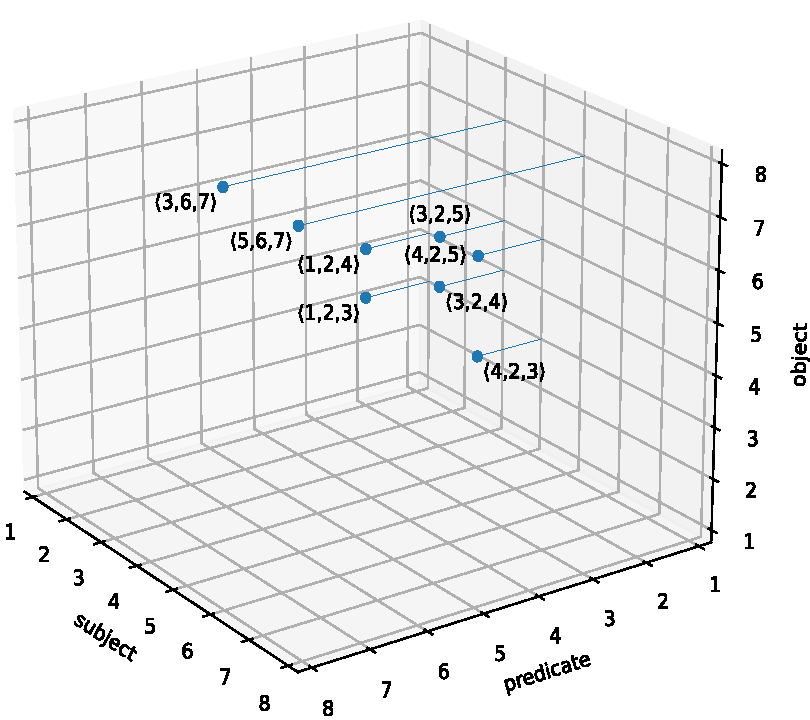
\includegraphics{figures/chapter2/3Dcoord-cut}
	\caption{A 3D plot of an order-3 RDF tensor representing the RDF graph in table \ref{tab:rdf_tensor}.}
	\label{fig:rdf_tensor}
\end{figure}

\subsubsection{Mapping SPARQL to tensors}
The ability to bridge SPARQL algebra to tensor operations is a strict requirement to realize a tensor-based triple store. For instance, a translation of triple pattern and basic graph pattern, core building blocks of SPARQL semantic, to tensor operations enables the triple store to evaluate queries based on those patterns, such as \verb|SELECT| queries. 

\paragraph{Triple Pattern} A slice of a tensor does basically what triple pattern does to the corresponding RDF graph. Thus, a triple pattern tuple $tp$ can be viewed as a slice key $s$ in the tensor domain. Slice positions ($\textbf{:}$) in $s$ are set at locations corresponding to the where variables are defined in $tp$.  Other locations in $s$ are set to concrete key parts (IDs) that maps to certain RDF terms defined in the tuple at the corresponding positions. Each variable in the triple pattern is associated with one dimension of the tensor. Now, evaluating a triple pattern $tp$ against an RDF graph $g$, is equivalent to slicing the tensor $T_{g}$ using slice key $s$. Then, the set of keys to non-zero elements in $S = T_{g}[s]$ are selected and the bounding key parts are assigned to the set of variables in $tp$ at the designated positions. \\


\begin{example}
	let $tp$ be a triple pattern defined as \verb|<?person ex:type ?type>| to be evaluated against the RDF graph $g$ in table \ref{tab:rdf_graph_example}.  An equivalent slice key $s$ for $tp$ is $s=$\verb|<:, 6, :>|. Slicing the RDF tensor $T_{g}$ (Fig. \ref{fig:rdf_tensor}) using $s$ results in an order-2 tensor with two non-zero entries (3, 7), (5, 7). Thus, the set of solution mappings is:\\ $\Omega = \{[?person \to res_{RT}(3), ?type \to res_{RT}(7)], [?person \to res_{RT}(5), ?type \to res_{RT}(7)]\}$.
\end{example}

\paragraph{Basic Graph Pattern}
Tentris relies on Einstein summation to evaluate basic graph patterns (BGPs). The idea is simple based on \cite{tentris2020}: "Triple patterns are resolved first and combined
via Einstein notation later using the variables of the triple patterns as labels subscripting
the operands (tensor slices). The result is subscripted with all used variables. The Einstein summation ensures that only non-zero entries of an operand are incorporated into
the result that matched with non-zero entries of the other operands only. Otherwise, values are set to zero as at least one of the operands resolves to zero".
\clearpage

\subsection{Tentris and Hypertrie}
\label{sec:hypertrie}
Underlying the order-d RDF tensor concept, Tentris realizes the concept using a novel data structure called Hypertrie. Before I discuss hypertrie structur, I first clarify how tensors storing RDF graphs can be represented as tries.\\

\subsubsection{Trie}
\label{sec:trie}
A \textit{Trie} \cite{Brass:2008:ADS:1434862} is a tree structure used to store \textit{sequences of characters} from an alphabet $\mathbb{A}$. An example of an alphabet is the ASCII codes set. Sequences, in this case, are strings. A node in a Trie contains potentially one outgoing edge for each possible character. Each node in the tree corresponds to a prefix of some sequences of the set, so if the same prefix occurs several times, there is only one node to represent it.\\

A possible realization of a Trie node is to use a pointer array of the size |$\mathbb{A}$| \cite{Brass:2008:ADS:1434862}. Each pointer points to either another trie node or null. Each array entry corresponds to a character in the alphabet. As an array lookup operation is computationally constant, looking up sequences in the Trie is fast and requires only $O(k)$ time where $k$ is the sequence size. However, this approach becomes space-inefficient as the size of the alphabet set increases or when it is infinite. An alternative way to store edges is to maintain a hash table $HT$ whose size will increase as we add distinct edges. The hash table keys correspond to \textit{edge labels} (characters) and are mapped to the node pointers (edges). Following that, the structure can still be used efficiently to retrieve sequences as accessing keys in a well-implemented sparse hash table is nearly constant. \\ 

A \textit{fixed-depth trie} $C$ is a trie that holds sequences of the same length $n$, termed as $keys$. In that case, a sequence $l = <l_0, … , l_m> \in \mathbb{A}^m$ of length $m <= n$ forms a \textit{key prefix}. $C[l]$ is defined as the node that is reached from the root node $r$ by walking along the nodes with edge labels equal to the entries of $l$. Hence, $C[l]$ could be undefined if no appropriate path exists. Moreover, \\

We can represent a tensor $T_g \in \mathbb{B}^{\mathbb{N}_n \times \mathbb{N}_n \times \mathbb{N}_n}$ that is used to store an RDF graph $g$ with |$RT$|$=n$ (Sec. \ref{sec:rdf_tensor}) using a fixed-depth trie $C_{T_g}$ of depth $d = $ ndim($T_g$) $=3$ with the alphabet $\mathbb{N}_n$. We call $C_{T_g}$ a \textit{a trie tensor or trie representation of $T_g$}, if: \\
\centerline{$\forall \textbf{k} \in \mathbb{N}_n \times \mathbb{N}_n \times \mathbb{N}_n, v \neq 0: T_g[k] = v \iff C_{T_g}[k] = v$}\\

Resolving a tensor trie $C_T$ of depth $d$ by key prefix $l = <k_0, ..., k_m>$ where $m<d$ is equavalent to slicing the corresponding $d$-order tensor using a slice key $s = <k_0, ..., k_m, e_{m+1}, ...,e_d>$ with $e_i$ = \textbf{:}. Then the resultant tensor slice $T[k_0, ..., k_m, e_{m+1}, ...,e_d]$ ($d^{'}$-order where $d^{'}=d-m$) is represented by an inner trie node or \textit{subtrie} of depth $d^{'}$. \\

In this writing context, the term \textit{node depth} corresponds to the length of the sequence that a node holds. For a trie tensor $C_T$ of depth $d$. The root node is assigned the depth $d$, an inner node holding prefix of size $m$ has the depth $d^{'}=d-m$. Leaf nodes share the depth 1. An example of a trie tensor is showed in figure \ref{fig:rdf_trie}.  \\

\begin{figure}[h]
	\centering
	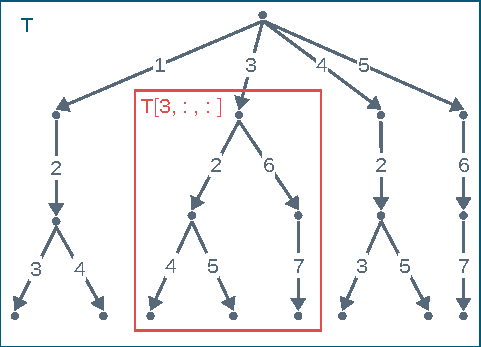
\includegraphics{figures/chapter2/trie4}
	\caption{Trie representation of the RDF tensor $T_g$ of the RDF graph $g$ in table \ref{tab:rdf_tensor}. A slice $T_g[3, :, :]$ by the first dimension with 3 is shown in the red (inner) box.}
	\label{fig:rdf_trie}
\end{figure}
\clearpage


\subsubsection{Hypertrie}
\label{sec:hypertrie_pre}
In the previous section we defined a trie as a data strucuture for realizing an order-3 RDF tensor. The structure is memory-efficient as it sparsely encodes a Boolean-valued tensor by storing only the keys that map to 1. As keys with the same key prefixes share the same node, a moderate level of compression is achieved. Slicing is also efficient if the set of edges to children are represented using a well-designed hashtable or search tree\cite{bras}. \\

A trie, as defined earlier, however, still lake the ability for flexible slicing, that is by any combination of dimensions. The trie tensor as it is defined so far allows slicing positions to only suffix the slice keys, thus using $s = <:, 3, :>$ as a slice key is not possible. Felxible slicing mush alwasy be maintained to enable resolving triple patterns (Sec. \myworries{???}). Tentris uses \textit{Hypertrie}, a novel trie-based data structure, for holding the keys of an RDF tensor. Hypertrie generalize the normal trie tensor concept by enabling the efficient slicing by any combination of dimensions. Hypertrie is defined formally based on Tentris paper \cite{tentris2020} in the following:\\

\begin{definition}
	\label{def:bht}
	Let $H(d, A, E)$ with $d \geq 0$ be the set of all hypertries with depth $d$, alphabet $A$ and values $E$.
	If $A$ and $E$ are clear from the context, we use $H(d)$.
	We set $H(0) = E$ per definition. 
	A hypertrie $h\in H(1)$ has an associated partial function $c^{(h)}_1: A\nrightarrow E$ that specifies outgoing edges by mapping edge labels to children.
	For $ h^{'} \in H(n), n>1 $, partial functions $c^{(h')}_i: A \nrightarrow H(d-1), i \in \mathbb{N}_{n}$ are defined.
	Function $c^{(h')}_i$ specifies the edges for resolving the part equivalent to depth $i$ in a trie by mapping edge labels to children.
	For a hypertrie $h$, $z(h)$ is the size of the set or mapping it encodes.
\end{definition}

Figure \ref{fig:rdf_hypertrie} shows a hypertrie storing the RDF triples shown in table \ref{tab:rdf_graph_example}. Examples for slicing hypertrie with different slice keys corresponding to various combinations of slicing positions is presented in figure \ref{fig:rdf_hypertrie_slice}. \\

\begin{sidewaysfigure}[h]
		\centering
		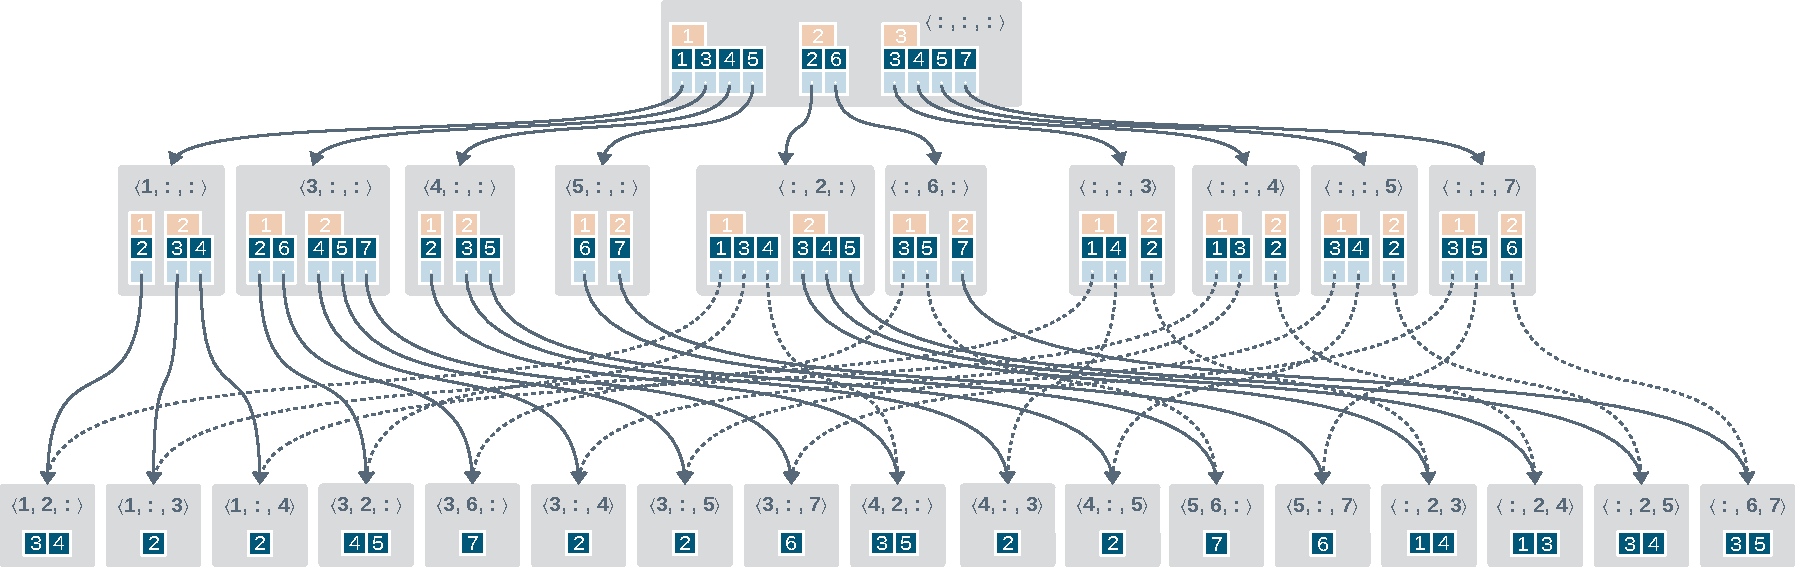
\includegraphics[scale=0.78]{figures/chapter2/hypertrie4}
		\caption{Hypertrie representation of the tensor $T_g$ in figure \ref{fig:rdf_tensor}. Each hypertrie node represents a tensor slice using the slice key presented in bold on the original tensor. Each node except for the leafs contain an array of hash tables each represents the set of edges at the corresponding key positions for the represented tensor. Scalar tensor nodes (leaf nodes) are printed as a set of key parts. The first reference to a child node is printed with a solid arrow, all further references are printed with a dashed arrow.}
		\label{fig:rdf_hypertrie}
\end{sidewaysfigure}

\begin{figure}[h]
	\centering
	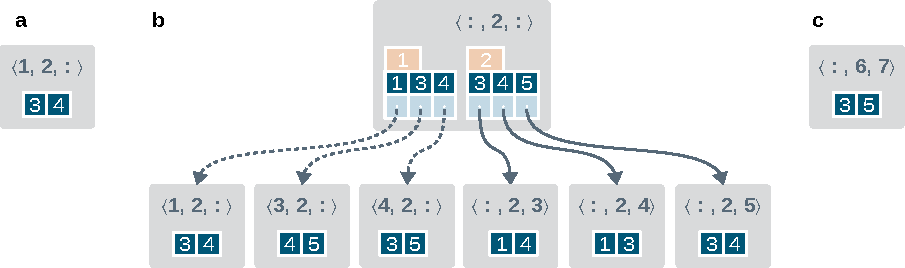
\includegraphics{figures/chapter2/hypertrie4_slices}
	\caption{Slicing a hypertrie using a tensor slice key can be done simply by following the path from the root node using the fixed key parts in the key in any combination at the corresponding positions. Nodes (a) and (c) are leaf nodes representing slicing an RDF tensor by a single slicing position. (b) is in an inner node that represents a 2D tensor slice.}
	\label{fig:rdf_hypertrie_slice}
\end{figure}
\clearpage